\documentclass[26pt]{article}
\usepackage[margin=2cm]{geometry}
\usepackage{amsmath, enumerate, graphicx, textcomp, caption, wrapfig, verbatim}
\usepackage{subcaption, listings, courier, fancyhdr, braille}
\lstset{basicstyle=\footnotesize\ttfamily, showstringspaces=false, showspaces = false, breaklines=true}
\usepackage{fancyhdr}
\graphicspath{{./images/}}
\newcommand{\tab}{\hspace*{2em}}
\newcommand{\n}{\newline}
\captionsetup[subfigure]{labelformat=empty}
\newcommand*{\code}{\fontfamily{pcr}\selectfont}

\title{Contextual Machine Learning Through the Analysis and Chunking of Partially Translated Grade 2 Braille}
\author{Catherine Ray}
\date{}
\begin{document}
  \maketitle

\pagestyle{fancy}
\renewcommand{\sectionmark}[1]{\markright{\thesection\ #1}}
\fancyhf{}
\rhead{\fancyplain{}{$Semester  Report$}}
\lhead{\fancyplain{}{\rightmark }} 
\cfoot{\fancyplain{}{\thepage}}
 
\begin{abstract}
I developed a machine learning program that uses contextual analysis algorithms to deduce the complex grammar rules of Grade 2 Braille given partially translated text. Using a known set of symbols (Grade 1 Braille), the parser translates the known symbols of Braille to English, and marks leftover unknown patterns and discrepancies. The parser matches unknown patterns to word groups and abbreviations. These learned patterns are stored in a persistent Map[String, TranslationOptions] format. 
\end{abstract}
\clearpage
\renewcommand{\abstractname}{Acknowledgements}
\begin{abstract}
I'd like to thank: Dr. Marr for introducing me to the beautiful complexity of Computational Semantics; Dr. Jahangeer for her amazing encouragement and her willingness to answer questions; Dr. Borne, Dr. Marr, and Dr. Papaconstantopoulos for supporting me and convincing me to major in Computational and Data Sciences; www.braillebookstore.com for printing and distributing books in Grade 2 Braille, excerpts of which helped train CAMEL.
\end{abstract}
\clearpage
\tableofcontents
\clearpage


\section{Introduction to Braille}


Standard Braille is an approach to creating documents which can be read through touch. As English words are composed of letters, Braille words are composed of Braille cells. A cell consists of six dots arranged in the form of a rectangular grid of two dots horizontally and three dots vertically. With six dots arranged this way, one can obtain sixty three different patterns of dots. The sixty-fourth pattern, a blank cell, represents a space. 

In addition to letters, the Braille alphabet includes combination of dots for punctuation, capitalization and numbers. In the Braille alphabet is depicted by a cell that contains six raised dots. The cell is divided into three rows of two columns. A letter is indicated by which dots are raised and which are smooth. Any letter can be capitalized by placing an indicator in front of the letter.

\textbf{Capitalization} is indicated by a cell with only the sixth dot, or the last dot of the cell in the lower right hand corner of the cell, raised while the rest are smooth. This cell appears in front of a letter cell to show capitalization. To capitalize an entire word, two cells with only the sixth dot raised in each cell is placed in front of the first letter of the word. \newline For example:  'ccc' = \braille{ccc}; 'Ccc' = \braille{Ccc}; 'CCC' = \braille{{Upper}ccc} \vspace{+10pt}

\textbf{Numbers} are represented using the first ten letters of the alphabet, "a" through "j", and a special number sign, \braille{{Number}}. This number sign is placed in front of a word to convert the entire word into numbers. If one wishes to switch from numbers to letters within a word (i.e. 212a) the letter sign, \braille{{Letter}}, is used.  \newline For example: 'cc' = \braille{cc}; '33' = \braille{{Number}cc}; '3c' = \braille{{Number}c{Letter}c} \vspace{+10pt}

\textbf{Contractions} are special characters used to reduce the length of words. English includes contractions (for example, "don't" is a contraction of the two words "do" and "not"). In Braille there are 189 additional contractions. Some contractions stand for a whole word. \newline For example: 'for' = \braille{{for}}; 'and' = \braille{{and}}; 'the' = \braille{{the}}. \vspace{+10pt} 
Other contractions stand for a group of letters within a word. In the example below, the contraction "ing" is used in the word "sing" and as an ending in the word "playing." Likewise, the contraction "ed" is used in the word "edge" and as an ending in the word "played." '\newline \{ing\} = \braille{{ing}} ; 's' + \{ing\} = \braille{s{ing}}; 'play' + \{ing\} = \braille{play{ing}} \newline \{ed\}  = \braille{{ed}} ; \{ed\} + 'ge' = \braille{{ed}ge}; 'play' + \{ed\} = \braille{play{ed}} \vspace{+10pt}

\textbf{Short-form contractions} are abbreviated spellings of common longer words. For example: "tomorrow" is spelled "tm", "friend" is spelled "fr", and "little" is spelled "ll" in Braille.  \newline

Translating the phrase "you like him" into uncontracted (a.k.a Grade 1 Braille) and contracted (a.k.a Grade 2 Braille), the effect contractions have on sequence length is evident. \newline
\braille{you like him} (Uncontracted) \newline \newline
\braille{{you} {like} hm}  (Contracted) \vspace{+10pt} \newline The reader is encouraged to see the appendices for further information on Grade 1 and 2 Braille translations. 

\subsection{Binary Braille}

The Braille alphabet is depicted by a cell that contains six raised/flat dots, numbered one through six beginning with the dot in the upper left-hand corner with the number descending the columns (see figure below).  In order to create a bitstring easily parsable by the computer,  "0" = flat, "1" = raised. The 3x2 matrix (Braille cell) is represented as a 1x6 bitstring (Binary Braille). \newline
\begin{tabular}{|l|l|}
\hline 1 & 4  \\ \hline 2&5 \\ \hline  3 & 6\\ \hline
\end{tabular} = \begin{tabular}{|l|l|l|l|l|l|}
\hline 1 & 2 & 3 & 4 & 5 & 6 \\ \hline
\end{tabular} ; Thus, "c" = \braille{c} $\equiv$ \begin{tabular}{|l|l|}
\hline $\cdot$ & $\cdot$ \\ \hline & \\ \hline  & \\ \hline
\end{tabular} $\equiv$ \begin{tabular}{|l|l|}
\hline 1 & 1  \\ \hline 0&0 \\ \hline  0 & 0 \\ \hline
\end{tabular} $\equiv$
\begin{tabular}{|l|l|l|l|l|l|}
\hline 1 & 0 & 0 & 1 & 0 & 0 \\ \hline
\end{tabular} $\equiv$ 100100




\section{Introduction to CAMEL}

CAMEL is an acronym of \textbf{C}ontextu\textbf{A}l \textbf{M}achin\textbf{E} \textbf{L}earning - with Braille as a language platform, this machine learning program uses the context of unknown symbols to deduce meaning and compress information. Provided the meaning of an initial set of symbols (a dictionary, or {\code dict}), CAMEL infers the meanings of unknowns and adds these meanings to the {\code dict}. Some symbols differ in meaning depending on their context. These translation options are stored in the {\code dict} in the form of {\code Map[String, TranslationOptions]}.


\subsection{String Processing Method}

CAMEL deduces the complex grammar rules of Grade 2 Braille given partially translated text. It learns new symbols by taking 2 input text files (Braille text and corresponding English text), and analyzing them until all unknowns are identified, their meanings are found, and said symbols and their meanings are added to the dictionary. 

\begin{figure}[ht!] \centering
	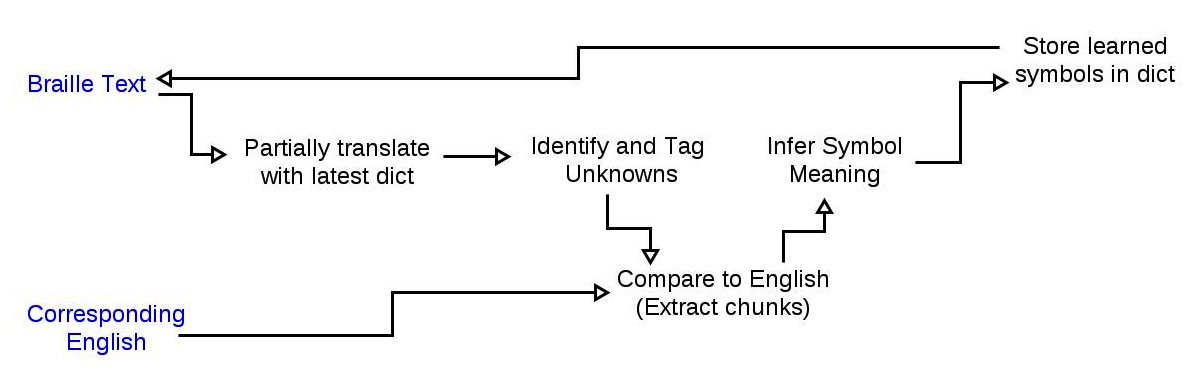
\includegraphics[width = 0.9\columnwidth]{Braillebig}
	\end{figure}

\subsection{Methods of Tagging and Text Extraction}

CAMEL must \textit{Tag Unknowns \& Compare to English(Extract Chunks)}  to infer symbol meaning. Four different tag types were used: end, front, mid, and full-word. Below are examples of how these different types of tags were each used to extract meaning. 
\begin{figure}[ht!]\centering
	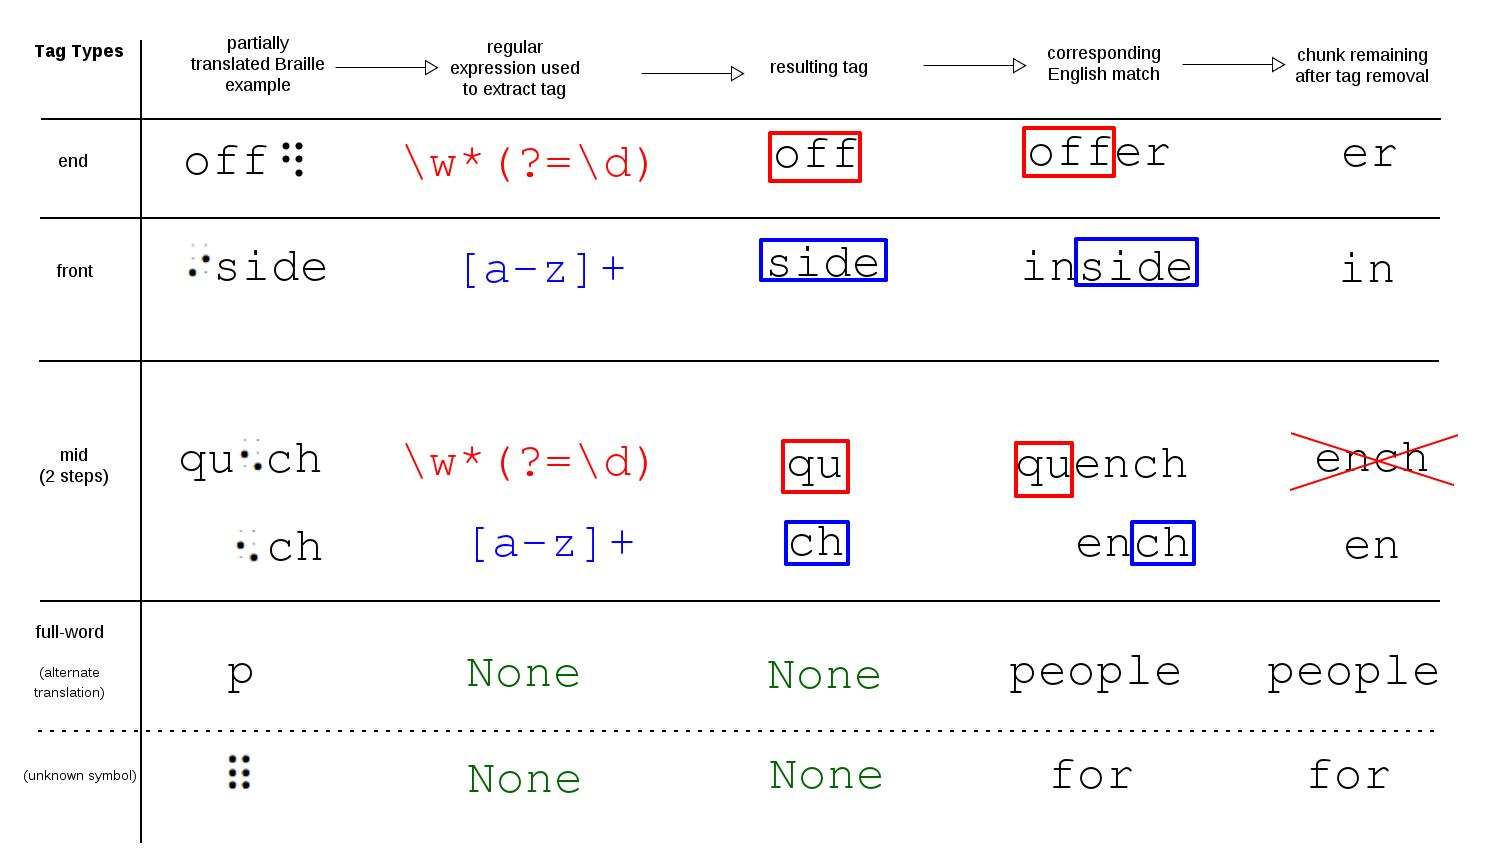
\includegraphics[width=0.9\columnwidth]{taggtypes1}
	\end{figure}
\clearpage

\subsection{Using Contracted Braille As a Platform}
Below is an example of the process of \textit{Tagging and Text Extraction}, in which CAMEL infers the symbols that represent \textit{en} and \textit{in} using the word \textit{penguin} (contracted to \textit{p\{en\}gu\{in\}} in Grade 2 Braille):
          \begin{figure}[ht!] \centering
	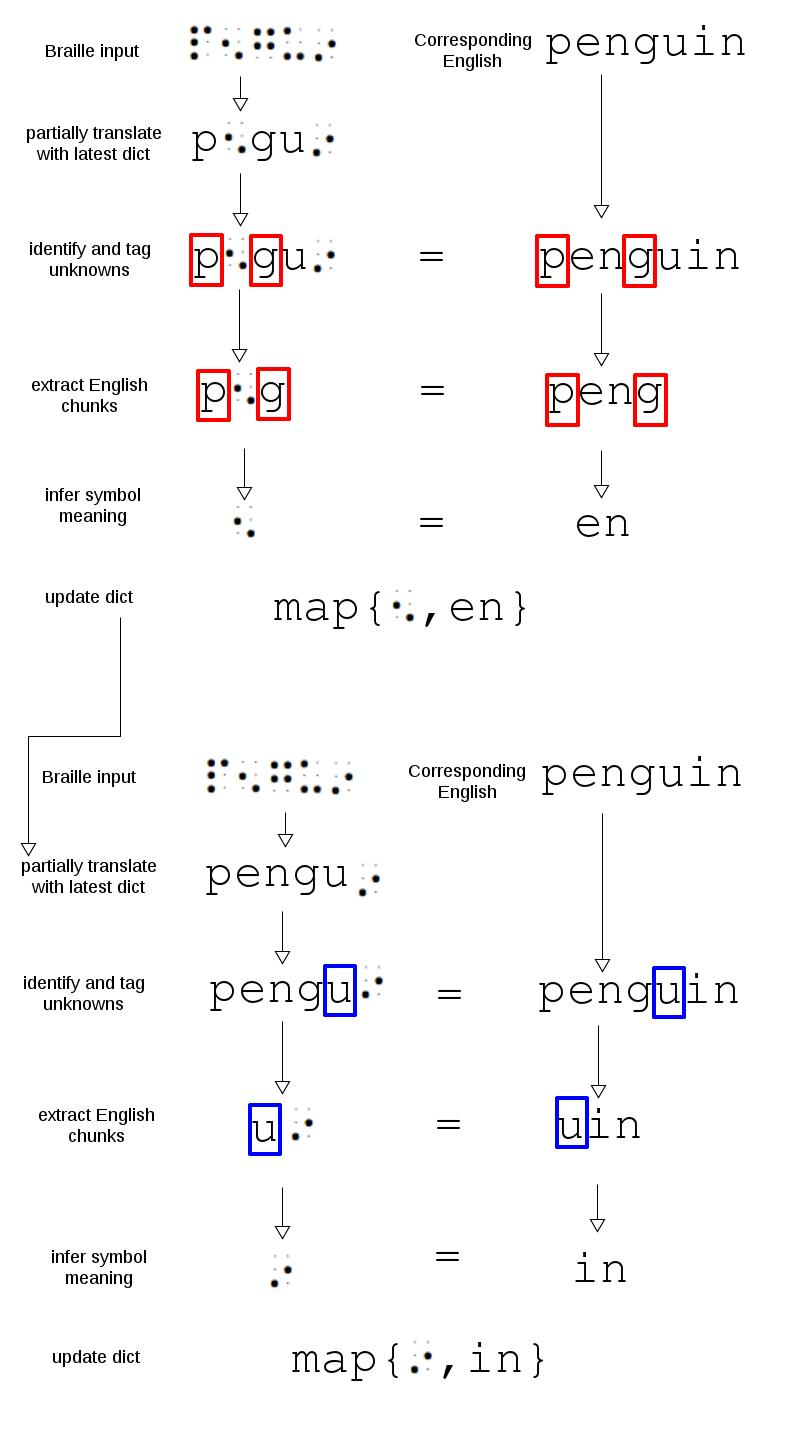
\includegraphics[width = 0.5\textwidth]{penguin-6}
	\end{figure}
\clearpage
\section{Evolution of the Program}

CAMEL was programmed in Python 2.7.3. This language was chosen because of the mutable nature of the {\code dict} constructor$^{[2]}$. Henceforth, this paper will refer to the set of symbols in Uncontracted Braille as "G1" and the set of symbols in Contracted Braille as "G2." 
%\clearpage
This table demonstrates (using arbitrary example inputs) the evolution of the program, version by version. \newline\newline
%\tabcolsep=0.11cm
\noindent
\resizebox{\linewidth}{!}{
\begin{tabular}{l| l | l | l | l}
%Monoatom results
{\tiny Version} & Input & (Partial)Translation & Output & Note\\
\hline\hline
0 & \braille{stop it} & {\code stop it} & & only accepts G1 input\\
\hline
1 & \braille{{st}op it} & {\code *op it} & & accepts G2 input\\
\hline
2 & \braille{{st}op it} & {\code *op it} & {\code st = *} & doesn't differentiate between unknowns\\
 & \braille{p{en}gu{in} has fl{ea}s} & {\code p*gu* has fl*s} & {\code eninea = ***}  \\
\hline
3 &  \braille{p{en}gu{in} has fl{ea}s} & {\code p\textbf{0}gu\textbf{1} has fl\textbf{2}s} & {\code en = \textbf{0}} = \braille{{en}} & differentiates between unknowns\\
&&& {\code in = \textbf{1}} = \braille{{in}}\\
&&& {\code ea = \textbf{2}} = \braille{{ea}}\\
\hline
4 & \braille{off{er} is p{ow}{er}}& {\code off\textbf{0} is p\textbf{12}} & {\code er = \textbf{0}} = \braille{{er}} & improves accuracy of inferred meaning\\
&& {\code offer is p\textbf{3}er} & {\code ow = \textbf{3}} = \braille{{ow}} \\
%\hdashline
& \braille{k is p{ow}{er}} & {\code k is power}& & retrieves unknowns to \\
&&&& improve partial translation \\
\hline
5 & \braille{k is p{ow}{er}} & {\code k is p\textbf{01}}& {\code ow = \textbf{0}} = \braille{{ow}} & detectsa and infers one-letter contractions \\
&& {\code k is pow\textbf{2}} & {\code er = \textbf{3}} = \braille{{er}} \\
&&  {\code k is power} & \braille{k} = \\
& & & \{{\code k} or {\code knowledge}\} \\
& \braille{{it} is k} & {\code x is knowledge}& {\code x} = \{{\code x [in word]} or {\code it}\}  \\
\hline
6 & \braille{{Capital}{Capital}{and} {Number}0234} & {\code 0 \textbf{0234}} & {\code and = \textbf{0}} = \braille{{and}} & capital letter and number functionality\\
\hline\hline
\end{tabular}}  \newline


\subsection{Uncontracted Braille-to-English Translator}
The first step was coding a functional program that translated raw G1 input into English text. Using a hard-coded Python {\code dict}, this was rather simple. CAMEL was given a {\code dict} containing only G1 symbols.

%Version0\lstinputlisting[language=Python]{code/B2T.py}

When the Braille input contained the string {\code 011100 011110 101010 111100 000000 010100 011110}, "stop it" was returned. \newline\newline This function can be represented in Python-esque psuedocode as follows.

\begin{lstlisting}
function (array of G2-words):
	translated_word = empty string
	for each word: 
		for symbols in word:
			symbol = dict[symbol]
			translated_word = translated_word + symbol
		translated_sentence[index of word] = translated_word
	return translated_sentence	

\end{lstlisting}


\subsection{Partial G2-English Translator}
Recall that G1 is uncontracted Braille. The set of G2 symbols consists of G1 symbols and additional contracted cells. Since the given {\code dict} consists only of G1 symbols, contracted cells are not recognized.

Recall that $G2 = G1 \cup \textnormal{Contracted Cells}$, thus $G1 \subset G2$. 
In Version0, if CAMEL processed a symbol that it did not recognize (i.e. symbol $\notin$  {\code dict}), a {\code KeyError} was thrown. This is due to the nature of Python {\code dict} constructors$^{[2]}$. 

In order to take G2 input and translate the known patterns, a try-except error catcher was added. The error catcher translated unknown cells as *.  

\begin{lstlisting}
function (array of G2-words):
	translated_word = empty string
	for each word: 
		for symbols in word:
			if symbol in dict: 
				symbol = dict[symbol]
			else: 
				symbol = *
			translated_word = translated_word + symbol
		translated_sentence[index of word] = translated_word
	return translated_sentence
\end{lstlisting}

%Version1\lstinputlisting[language=Python]{code/B2T0.py}

When 'braille.txt' contained the string {\code 001100 101010 111100 000000 010100 011110}, {\code *op it} was returned. The string {\code 001100} $\equiv$ "st" in G2, but "st" $\notin$ G1, and was consquently represented as an asterisk. 

\subsection{Matching Partial G2-English Translation to Corresponding English Chunks}
 We must be able to remove duplicates from sets whilst keeping order. The Python {\code set} is an unordered collection with no duplicate elements. We need an ordered collection with no duplicate elements, so another method is introduced.\newline I will feed Version2 "stop it = *op it", and Version must see that *=st, for all other characters are accounted for. I did this by taking the {\code translated\_sentence}.

\begin{lstlisting}
function (translated sentence)


\end{lstlisting}


%Version2\lstinputlisting[language=Python]{code/B2T1.py}

When 'braille2.txt' contained the string "001100 101010 111100 000000 010100 011110", evaluated by the 'translate' method as $\equiv$ "*op it", and 'eng2.txt' contained the string "stop it".  "st = *" was returned! \n Given two inputs \n input1 = "stop it"  \n input2 = \braille{{st}op it} \n

The program translates input2 using the given G1 dictionary. However, input2 has symbols not in the G1 dictionary, thus these symbols are left untranslated.  input2 = \braille{{st}op it} $\rightarrow$ output1 = \braille{{st}} op it 

Given that input1 = input2, and input2 = output1 the program compares the overlap between input1 and output1 to find the most likely meaning of the unknown symbol.
"stop it" = \braille{{st}} op it $\Rightarrow$ \braille{{st}} $\equiv$ "st"

Summarized, Version2 does the following:\n "stop it" = \braille{{st}op it} $\rightarrow$ \braille{{st}} op it $\Rightarrow$ \braille{{st}} $\equiv$ "st" 
\newline\newline 



\subsection{Storing and Retrieving Unknowns to Improve Partial Translation}

This seemed to work wonderfully, but when applying Version1 to the English phrase "penguin has fleas." The partially translated string $\equiv$ "p*gu* has fl*s" was created; this gave "eninea = ***" as the output. This finds the English chunks, but doesn't differentiate between the unknowns.

In order to differentiate the unknowns, the program was altered such that the asterisks were replaced with numbers. Thus, instead of "p*gu* has fl*s", we differentiate the unknowns as "p0gu1 has fl2s."  Furthermore, regex was used to extract the flags before and after each digit. So, "0" was preceeded by "p" and followed by "g", when this search was applied to "penguin", the "en" was extracted. Success, and the birth of Version3 (mostly edits to the translate method). 
Once the unknowns were successfully stored, they were utilized by the program. \newline\newline This version takes into account the following tags (see Introduction to CAMEL[2.2]) \newline (1) Letters before and after the unknown\newline(2) Letters after the unknown\newline(3) Letters before the unknown\newline(4) Unknown alone
\newline\newline 


\subsection{Matching Separate Occurances of Unknowns to Infer Meaning}

This version (Version4) looks at consequent unknowns. For example, the G2 braille form of "offer is power" is "off\{er\} is p\{ow\}\{er\}." Note that \{er\} is present in two seperate occurances, additionally, \{ow\} and \{er\} are consequent. 

\braille{off{er} is p{ow}{er}} $\rightarrow$ off\braille{{er}} is p\braille{{ow}{er}} 

This is taking "power" = 'p10', and returning 1 = "ower", 0 = "er"; this error is eliminated by retranslating the input each time a new unknown was found.
\newline\newline 

\subsection{Storing Translation Options in Map[String, TranslationOptions] Format}
This required use of the known text to match TranslationOptions to the given English text. For example, the pattern {\braille {bb}} is used for both "bb" and "be". Thus, once the computer infers a meaning, the computer will translate other instances of this pattern incorrectly. Using the structure of a Python {\code dict}, it is simple to add options for keys. \newline\newline   This version takes into account the following tags (see Introduction to CAMEL 2.2) \newline (1) Letters before and after the unknown\newline(2) Letters after the unknown\newline(3) Letters before the unknown\newline(4) Unknown alone\newline(5) Known alone (a.k.a. translation options for one-letter contractions)
\newline\newline



The first instance of this I dealt with is one word contractions. The output of Version5 was\newline110111 = er\newline010101 = ow\newline\newline Input: offer knowledge is power \newline\newline Output: offer k is power \newline\newline One letter contractions exist:
k means knowledge in this context.\newline\newline In Version5, I mainly optimized the system of detecting translated letters vs. untranslated ones. 

The context in which "k" = knowledge is found is The source code used to implement this algorithm is in Source Code[7.6].

\subsection{Adding Functionality}

In order to include number and capitalized letter functionality, new checks were added to the translate method. \newline

\subsection{Optimizing the Program}

In order to save time and processor power, a generator was used (instead of an iteratable array) when printing partially translated text.

Using regular expressions (instead of repeatedly searching combinations of the array indices) improved the time and accuracy of English chunk extraction.

\section{Results and Conclusions}

\subsection{Safety of Community}
\begin{itemize}
		\item commercial application in development that will prevent future mislabeling,  such as
	\begin{figure}[ht!]\centering
	
\includegraphics[width = 0.5\textwidth]{stairwellmis}
	\end{figure}
 		\item allows sighted people to protect the blind community
\end{itemize}

\subsection{Proof of Concept} 
             \begin{itemize}
    		\item $1^{st}$ succesful automated program that learns compressed Braille
		\item translation system is effective for arbitrary symbol systems 
		\item language platform easily changed
		\end{itemize}

CAMEL is the $1^{st}$ succesful automated program that learns compressed Braille. This translation system is effective for arbitrary symbol systems, and the language platform easily changed.

\subsection{GUI}
For users not familiar not comfortable with the binary representation of Grade 2 Braille, a GUI option was created. This immediately converts from a graphical braille representation into a binary string for CAMEL to parse.

This program could be expanded to an application for sighted-people not familiar with braille. Instead of manually entering Braille with the GUI system, a user could point their phone's camera at the Braille string they wish to translate, and image processing techniques could identify the Braille listed. This Braille would be translated using the dictionary generated by CAMEL.

\subsection{Further Research}
The method of detection for one letter contractions is comparing the original text, not checking likely matches for the one-letter contractions in a weighted sentence dictionary. CAMEL implements word-level analyzation, and could be improved by using sentence-level analyzation. 

The results of this project are the foundation for a usable app (Section[4.3]), for the sighted to decode Braille writing.

\clearpage

\section{Documentation for CAMEL}


%Function: Multiply

%Multiplies two integers.

%Parameters:
	%x - The first integer.
	%y - The second integer.

%Returns:
	%The two integers multiplied together.

\textbf{Function}: {\code translate}

Translates known characters, assigns integers to unknown characters. \newline\textbf{Parameters}: 

{\code brl\_array} - array of binary strings, one string per index
\newline\textbf{Returns}:

(Partially-)translated string.\vspace{+20pt} \newline\textbf{Function}: {\code file2array}

Extracts text from file into parsable format.
\newline\textbf{Parameters}: 

{\code filename} - name of the file from which to extract the strings 
\newline\textbf{Returns}:

array of strings, one word per index (whitespace is used to determine word seperation)\vspace{+20pt} \newline\textbf{Function}: {\code matching}
%Tags and extracts English chunks to infer symbol meaning, updates {\code dict} with learned symbols, and recursively translates until all the meanings of all unknown symbols are inferred and stored correctly.

Recursively infers and stores (updates {\code dict}) the meanings of unknown symbols. \newline\textbf{Parameters}: 

{\code partially\_translated\_text} - array of partially translated words, one word per index
\newline\textbf{Returns}:

Recursive output of {\code translate} using the updated {\code dict} \vspace{+20pt} \newline\textbf{Function}: {\code testing}

Searches for, identifies and translates capitals, numbers, and one-letter contractions.
\newline\textbf{Parameters}: 

{\code new\_translation} - newest translation of input
\newline\textbf{Returns}:

None\vspace{+20pt}
\newline \textbf{Function}: {\code weight} (\textit{in progress})

Weights the translation options from the given symbol's {\code dict} entry using the context of the sentence.
\newline\textbf{Parameters}: 

{\code dict\_symbol} - {\code dict} entry for given symbol

{\code brl\_array} - array of binary strings, one string per index
\newline\textbf{Returns}:

Most likely translation of a given symbol.\vspace{+20pt}

\section{Source Code}

Version6
\lstinputlisting[language=Python]{code/B11.py}

\begin{comment}
\section{Source Code (Versions [0-5])}

\subsection{Version0: Uncontracted Braille-to-English Translator}
Version0\lstinputlisting[language=Python]{code/B2T.py}


\subsection{Version1: Partial G2-English Translator}
Version1\lstinputlisting[language=Python]{code/B2T0.py}

\subsection{Version2: Matching Partial G2-English Translation to Corresponding English Chunks}

Version2\lstinputlisting[language=Python]{code/B2T1.py}


\subsection{Version3: Storing and Retrieving Unknowns to Improve Partial Translation}

Version3\lstinputlisting[language=Python]{code/B2T3.py}


\subsection{Version4: Matching Separate Occurances of Unknowns to Infer Meaning}

Version4\lstinputlisting[language=Python]{code/B2T3.py}


\subsection{Version5: Storing Translation Options in Map[String, TranslationOptions] Format}
Version5\lstinputlisting[language=Python]{code/B2T8.py}
\end{comment}
%\subsection{Version6: Adding Functionality}

%Version6\lstinputlisting[language=Python]{code/B11.py}




%Conceptual compression, embedded in the fact that between Braille 1 to Braille 2 there is a symbolic reduction.

%Physical Symbol System Hypothesis PSSH
%Commerical operation, coding has begun - NSF Saftety protecting people from wrong information that could led to physical damage. Rapidly determine if signs could lead to physical problems.


\appendix
\section{Braille Alphabets}
\includegraphics[width=0.85\textwidth]{i/Step1}
\section{Prefix Indicator}
\includegraphics[width=0.4\textwidth]{i/PrefixIndicator}
\section{Contraction for Part of Word}
\includegraphics[width=0.85\textwidth]{i/ContractionForPartofWord}
\section{Final Letter Contraction for Middle or End of Word}
\includegraphics[width=0.6\textwidth]{i/FinalLetterContractionforMiddleorEndofWord}
\section{Initial Letter Contraction for Whole or Part of Word}
\includegraphics[width=0.85\textwidth]{i/InitialLetterContractionforWholeorPartofWord}
\section{Abbreviation for Whole Word}
\includegraphics[width=0.85\textwidth]{i/AbbreviationfortheWholeWord}


\section{Bibliography}

[1] http://texdoc.net/texmf-dist/doc/latex/braille/summary.pdf\newline
[2] http://docs.python.org/2/library/stdtypes.html\#dict

\end{document}

Yes, I think about what could of been if I'd stayed at Mary Baldwin. I'd definitely have more friends, and I'd be taking more advanced classes.


